\documentclass[11pt]{article}

\usepackage{amsmath}
\usepackage{graphicx}
\usepackage{multicol}
\usepackage{wrapfig}
\usepackage{hyperref}
\usepackage{tabularx}
\usepackage{setspace}
\usepackage{comment}
\usepackage{color}
\usepackage{pdfpages}
\usepackage[table]{xcolor}

%\usepackage{natbib}
\newcommand\citep{\cite}
\newcommand\citet{\cite}

\oddsidemargin 0cm
\evensidemargin 0cm

\usepackage{tocloft}

\setlength\cftparskip{6pt}
\setlength\cftbeforesecskip{4pt}
\setlength\cftaftertoctitleskip{2pt}

\usepackage[compact]{titlesec}  
\titlespacing{\section}{0pt}{0pt}{-5pt}
\titlespacing{\subsection}{0pt}{0pt}{-8pt}
\titlespacing{\subsubsection}{0pt}{-5pt}{-8pt}

\oddsidemargin 0cm
\evensidemargin 0cm

\usepackage[margin=1in]{geometry}


\parindent 0cm
\parskip 0.5cm

\linespread{1.1}

\usepackage{fancyhdr}
\pagestyle{plain}
%\fancyhf{}
%\fancyhead[L]{AOSS Reference Sheet}
%\fancyhead[CH]{test}
\fancyfoot[C]{Page \thepage}

\newcommand{\vb}{\mathbf}
\newcommand{\diff}[2]{\frac{d #1}{d #2}}
\newcommand{\diffsq}[2]{\frac{d^2 #1}{{d #2}^2}}
\newcommand{\pdiff}[2]{\frac{\partial #1}{\partial #2}}
\newcommand{\pdiffsq}[2]{\frac{\partial^2 #1}{{\partial #2}^2}}
\newcommand{\topic}{\textbf}
\newcommand{\arcsinh}{\mathrm{arcsinh}}
\newcommand{\arccosh}{\mathrm{arccosh}}
\newcommand{\arctanh}{\mathrm{arctanh}}

\renewcommand\refname{}

\begin{document}

\pagenumbering{roman}

\begin{center}
{\large \textbf{TempestExtremes: Indicators of change in the \\ characteristics of extreme weather}}

Dr. Paul Ullrich (PI) \\
\textit{Department of Land, Air and Water Resources, UC Davis}

Dr. Richard Grotjahn (Co-PI) \\
\textit{Department of Land, Air and Water Resources, UC Davis}

Dr. Colin Zarzycki (Co-I) \\
\textit{National Center for Atmospheric Research}
\end{center}

\begin{spacing}{-1.0}
\tableofcontents
\end{spacing}

\clearpage

\setcounter{page}{1}
\pagenumbering{arabic}

\section{Scientific / Technical / Management}

\subsection{Motivation and Objectives}

This research proposal targets \textbf{NASA Strategic Research Objectives} (ROSES-2014) ``\textit{Climate Indicators and Data Products for Future National Climate Assessments}.''  This proposal incorporates aspects of both \textit{Climate Indicators}, by developing and improving indicators based on characteristics of extreme weather events, and \textit{Assessment capabilities and products}, by supporting the development of a new software pipeline for the analysis of data sets and model output.

\vspace{-10pt}
\paragraph{Overview:}  The next century will see unprecedented changes to the climate system, which are in turn expected to drive changes to the characteristics of meteorological extremes. These changes will have direct impact on populations throughout the United States: As stated by third National Climate Assessment (NCA), ``changes in extreme weather and climate events, such as heat waves and droughts, are the primary way that most people experience climate change.'' The characteristics of extreme weather are key climate indicators, and addressing observed (lagging) and projected (leading) changes in these quantities will be important across multiple sectors, in multiple regions, and highly useful input to future NCAs.  This project will address the pressing need for a better understanding of changing extremes, including tropical cyclones (TCs), extratropical cyclones (ETCs), atmospheric blocks, atmospheric rivers (ARs), temperature extremes and precipitation extremes. 

\vspace{-10pt}
\paragraph{Objectives / Tasks:}  The \textbf{central objective} of this proposal the provision of an assessment of trends in the \textbf{characteristics of extreme weather events} observed over the past century.  The \textbf{secondary objective} of this proposal is to provide a new \textbf{assessment capability} in the form of an \textbf{automated pipeline for detection and characterization of extreme weather events}.  These objectives are expanded as four research tasks: 
\vspace{-10pt}
\begin{itemize}
\item[(T1)] Implement expanded functionality for detection and characterization of atmospheric blocks, atmospheric rivers, extreme temperature and extreme precipitation events in the extreme weather detection/characterization framework TempestExtremes.

\item[(T2)] Assess differences in new and existing detection and characterization algorithms.  Using reanalysis and model data, provide a comprehensive assessment of past changes in the characteristics of these extremes.

\item[(T3)] Using large ensemble simulations from the Climate of the 20th Century (C20C) project, determine how the characteristics of extreme weather events under historical climate simulations differ from hypothetical climate simulations with preindustrial greenhouse gas concentrations.

%\item[(T4)] Using CLIVAR experiments and CMIP5/6 model output, provide an assessment of predicted changes in the characteristics of extreme weather events.

\item[(T4)] Through the NASA Earth Exchange (NEX), provide scientists with the capability for automatic analysis of datasets using a suite of detection and characterization algorithms. 
\end{itemize}

%This work will emphasize regional and local-scale changes in extreme events.

\subsubsection{Central Theme: Discrete Extreme Weather Events}

This proposal targets a broad class of regional-scale \textbf{extreme weather} events that appear in climate datasets, with a particular emphasis on the North American continent.  These events include both ``nodal'' features with a specific geographic location, such as the sea-level pressure minimum associated with extratropical cyclones and tropical cyclones, and features ``areal'' features, including atmospheric rivers, atmospheric blocks, heat waves and precipitation extremes.  All events have both a spatial location / extent and a temporal component, including a distinct start and end time.  Extreme weather events include both propagating events (those that gradually change spatial position over time) and stationary events.  The \textbf{climate indicators} targeted by this proposal are the characteristics of these features, and are itemized in section \ref{sec:ExtremeWeather}.

\subsubsection{Central Theme: Big Data}

Over the past century there has been an explosive growth in the number of meteorological observations, more recently augmented by multi-terabyte datasets from climate models and climate analysis.  Analysis of this vast reservoir of climate data is a pressing challenge for climate researchers over the next decade \citep{levy2012bigdata, ganguly2008data}.  Forthcoming high-resolution global atmospheric simulations at scales of 10km will each require roughly a petabyte of active storage, and post-processing of this data will be an inevitable bottleneck in the process of understanding regional climate change.  The need for rapid high-throughput data analysis tools that have been validated on climate data is now greater than ever.  Current technologies include a smorgasbord of competing algorithms for detection and characterization that typically address only a single type of extreme weather, frequently require disparate input data formats and generally only work for data on a specific type of grid \citep{neu2013imilast}.  Consequently, the proposed work has the potential to dramatically simplify and streamline the process of detection and characterization of synoptic scale phenomena in large-scale climate datasets, and so will lead to a better understanding of how these features are represented within climate simulations.

\subsubsection{Impact}

According to the Intergovernmental Panel on Climate Change (IPCC), since 1980 annual losses from extreme weather events have ranged from several billion to over 200 billion.  Weather-related disasters have also caused a significant loss of human life over the past century, including nearly 500,000 deaths from the Bhola Cyclone in Bangladesh (1970), over 1,000,000 deaths from the 1931 central China floods, and 70,000 deaths from the European heat wave of 2003.  Consequently, we argue that an understanding of how extreme weather events have changed as a consequence of human influence is a pressing requirement of any climate assessment.

The assessment extreme weather characteristics that is the focus of this work will augment existing studies that have only targeted specific types of extreme weather event or have only dealt with singular datasets.  The advantage of considering multiple event types under a single umbrella allows for analysis and identification of connections between these phenomena.  For instance, atmospheric blocking in the Eastern Pacific is responsible for redirecting atmospheric rivers, which in turn leads to a modification of precipitation patterns.  The use of multiple datasets and the development of a pipeline for data analysis will improve our statistical confidence in observed trends and provide a mechanism for scientists to rapidly analyze new climate datasets.

\subsubsection{Relevance for NASA}

This project aims to fill in many of the gaps that exist within the last National Climate Assessment (NCA) associated with extreme weather events, and improve our confidence in reported trends for existing extreme weather studies.  The development of a climate data analysis pipeline for extreme weather will position NASA as a cornerstone agency for the analysis of climate data from national and international sources, and will assist in the analysis of future climate data products produced from future NASA missions.  In accordance with the RFP, this project also aims to increase the number of researchers performing assessment-relevant science via training of two graduate student researchers (GSRs).

{\color{red} NASA also has an ongoing effort to develop and improve climate datasets. Accordingly, this proposal includes a component of verification of MERRA � for specific applications for which it has not yet been tested.}

%\subsubsection{Global Impact}

%This proposal aims to not only build on the previous work of the international community via integration of internationally developed datasets, but also aims to have a broad global impact.  Blocking events have been particularly disastrous throughout Europe and Russia in the past several decades (especially from the 2003 European heat wave and 2010 Russian heat wave), and global change threatens to worsen these events.  Extratropical cyclones have also been devastating, especially in northern Europe and the British Isles, but major storms associated with extratropical cyclones have also caused significant damage to New Zealand (1968) and Uruguay (2005).  Since this work focuses on leveraging high-throughput data analysis methods for global climate data, it is natural to consider these extreme events from a global perspective.  The results of this work will be shared with international collaborators in Europe and beyond, and will aid in developing effective mitigation and adaptation strategies against changing climate events.


\subsection{Extreme Weather Events, Sectors, Regions, and Indicators} \label{sec:ExtremeWeather}

This section provides a brief overview of each of the extreme weather events that will be targeted by this proposal along with affected sectors and regions.  The key characteristics (indicators) that will be identified and catalogued for each feature are provided.

\subsubsection*{Tropical Cyclones (TCs)}

Tropical cyclones (TCs) are severe storms originating in warm, tropical, ocean basins which are characterized by their strong surface winds and low pressure center. Storm sizes can range anywhere from 100 km to over 4,000 km in diameter. Landfalling TCs produce intense winds, heavy rain, high waves, and damaging storm surge in coastal locations \citep{EmanuelDivineWind}. They are currently estimated to be responsible for 19,000 fatalities per year and \$26 billion/year in damages worldwide \citep{Mendelsohn2012}, making them one of the most devastating natural phenomena.

%TCs are referred to regionally as tropical storms, hurricanes (Western Hemisphere) and typhoons (West Pacific). In other locales, they are also called cyclones or cyclonic storms. 

%{\color{red}[Detection and Characterization of TCs?]}

Key sectors affected by tropical cyclones include energy, urban environments and transportation, primarily via infrastructural vulnerability.  Regions affected by TCs include the southwest, southeast and northeast, particularly along the coasts.

Key characteristics targeted by this proposal include seasonal counts, wind intensity, radius of maximum wind, precipitation intensity, total overland precipitation and spatial distribution of tracks.

\subsubsection*{Atmospheric Blocking}

Formally, atmospheric blocking is a meteorological phenomenon defined by an anti-cyclonic quasi-stationary high-pressure system persisting for several days to weeks and so is associated with negative vorticity anomalies in the Northern hemisphere (positive in the Southern hemisphere) and positive geopotential perturbation.  Blocking events are well characterized in the literature \citep{benzi1986anomalous}, and their connection with prolonged extreme temperatures is well known.  Sustained extreme temperatures, including heat waves and cold spells, which arise from atmospheric pressure blocking have been responsible for significant socioeconomic damage.  Historically, heat waves due to pressure blocking have led to thousands of deaths  in only the past decade, including roughly forty thousand casualties from the 2003 European heat wave \citep{bouchama20042003}, 220 deaths from the 2006 North American heat wave and over fifteen thousand casualties from the 2010 Russian heat wave.  In 2013, over 760 people died as a consequence of a long-running heat wave in Britain \citep{upi2013article}.  Additional losses from the North American heat wave were caused by drought conditions that spurred widespread forest fires, as well as large-scale convective storm events including the 2012 North American Derecho.  The economic cost of these events has been estimated to be in the tens of billions of dollars.

%The proposed work also leverages a large ensemble of previously unavailable climate simulations which are consistent with the observed and pre-industrial climate, and so has the potential to address the scientific questions in a rigorous statistical manner.

Key sectors affected by atmospheric blocking include water, energy, agriculture and human health.  In particular, persistent weather conditions caused by atmospheric blocks can affect precipitation patterns and lead to increases in local and regional air pollution.  Within the US, the northwest, southwest and Alaska are strongly affected by Pacific blocks which can redirect precipitation from the Pacific away from the coast.  The Great Plains, midwest, northeast and southeast are also affected by omega blocks, which are responsible for a range of extreme weather phenomena such as tornadoes and winter storms.

Key characteristics include intensity (for instance measured by the strength of the anomaly), lifetime, genesis location and track.

\subsubsection*{Extratropical Cyclones (ETCs)}

ETCs are phenomena associated with transient low-pressure systems occurring in the mid-latitudes of both hemispheres, and are sometimes known for producing damaging levels of wind, precipitation, low temperatures, and flooding \citep{serreze1995climatological, ulbrich2009extra}. In the span of a few hours, ETCs can travel across large areas and develop into massive storms resulting in widespread losses. Intense ETC events, such as the 1993 ``Storm of the Century'' in the eastern United States and the 1999 Windstorm Lothar in northern France, can cause hundreds of fatalities and significantly impact residential, commercial, and agricultural structures.

Key sectors affected by extratropical cyclones include energy, transportation, urban environments and human health.  Infrastructural vulnerabilities to extreme winter snowfall remains a persistent issue, but  cold temperatures and the effects of winter weather can also affect energy demand and human health.  Within the US, extratropical cyclones primarily affect the Northeast, Great Plains and Midwest regions.

Key characteristics include wind intensity, radius of maximum wind, precipitation intensity, total overland precipitation, proportion of precipitation as snowfall, and spatial distribution of tracks.

\subsubsection*{Atmospheric Rivers (ARs)}

ARs are meteorological phenomena characterized by long, narrow plumes of increased atmospheric moisture stretching between the subtropics and the midlatitudes regions \citep{ralph2011storms}.  These features are responsible for 30\%-50\% of total US west coast precipitation, particularly during winter months, and 30\%-40\% of total seasonal snow water \citep{dettinger2011atmospheric, warner2012wintertime}.  ARs are usually between 400 to 600\ km wide, and so at global model resolutions of $1^\circ$ are mostly unresolved, occupying as few as four grid cells in the latitudinal direction.  Those ARs with highest moisture content and strongest winds can induce extreme rainfall and can lead to flooding.  Notable AR events include the 2010 ``Snowmageddon'' event \citep{halverson2010mega}, responsible for record-breaking snowfall in the US northwest and the 1986 February atmospheric river that resulted in 13 fatalities, 50,000 people displaced by flooding and \$400 million dollars in damage \citep{leung2009atmospheric}.

%{\color{red} Make sure to cite Ralph and }

%doi: 10.1111/j.1752-1688.2011.00546.x  - 7 model ensemble of historical climate and future climate simulations, showing no change in average AR statistics, but a significant change in extremes:  years with many AR episodes increase, ARs with higher water vapor content increase, peak season for ARs will lengthen

%doi: 10.3390/w3020445  - California is very variable, and appearance of ARs can lead to drought or flooding conditions

%doi: 10.1002/2014GL060299  - with short lead times weather forecasting models perform well at predicting ARs over central US, but not skillful at 7 days.

%{\color{red}[Atmospheric river literature]}

Key sectors affected by atmospheric rivers include water, energy and agriculture, particularly for their role in the water cycle along the US West Coast, but these features are nonetheless relevant throughout the US.

Key characteristics include wind speed, total column integrated water vapor, precipitation intensity and point of landfall.

\subsubsection*{Extreme Heat Events (EHEs)}

{\color{red}[More here]}

Specific heat wave events have also been studied:  for instance, \cite{dole2011grl} use observational data to characterize human-induced influences on the 2010 Russian heat wave.  

Key sectors affected by extreme heat events include energy, agriculture and human health.  Energy infrastructure is particularly susceptible to extreme heat outbreaks, largely due to the increased energy demand required for air conditioning.  Extreme heat can also devastate crop yields and, in conjunction with high humidity, is a major cause of heat stroke and fatality among young children and the elderly, especially in disadvantaged communities.  All regions of the US are affected by extreme heat events.

Key characteristics include duration of heat events, apparent temperatures during heat events, overnight recovery temperatures and spatial extent.

\subsubsection*{Extreme Precipitation Events (EPEs)}

{\color{red}[More here]}

Key sectors affected by extreme precipitation events include water, energy, transportation and agriculture.  All regions of the US are affected by extreme precipitation events.

Key characteristics include ...

%Key Historical NASA  NASA reanalysis products will be key to assess past changes, including the Modern Era Retrospective-analysis for Research and Applications (MERRA) and North American Regional Reanalysis (NARR) (for all extreme events), NASA Earth Exchange (NEX) Downscaled Climate Projections, Daymet reanalysis (for temperature and precipitation extremes) and PRISM precipitation data (for precipitation extremes).

\subsection{Datasets} \label{sec:Datasets}

For the set of extreme weather events targeted by this proposal, accurate detection and characterization requires spatially gridded datasets with at least daily temporal resolution.  For features which are governed by the large-scale circulation, 6-hourly or higher temporal resolution is required.  Consequently, the key datasets for analysis will include MERRA, CFSR and ERA-Interim global reanalysis products, NARR regional reanalysis, and C20C ensemble simulations.  CMIP5 hindcasts covering the period 1979-2008 will be used to determine if observed trends are also present in climate model simulations.  For temperature and precipitation extremes, daily output will be used from Daymet and PRISM.

Follow-up efforts targeting leading indicators will also leverage CLIVAR experiments, which include multi-year static climatologies with (a) present-day greenhouse gas concentration and sea-surface temperatures (SSTs), (b) doubled atmospheric CO2 concentration (2xCO2), (c) increased global sea-surface temperatures by 2 degrees (SST+2) or (d) a combination of (b) and (c).  Future projections from CMIP5 (and upcoming sixth assessment) will also be used to assess trends in relevant indicators over the coming century.

\subsubsection*{MERRA / CFSR / ERA-Interim / C20C} \label{sec:MERRA}

Reanalysis products represent climate model hindcasts which are tightly constrained to known observational data.  More than a dozen global and regional reanalysis products are now available.  However, these datasets have the potential to differ significantly depending on the choice of model,  model parameters, the number and type of observations and the methodology by which data is assimilated into the model.  The focus of this proposal is on MERRA \citep{rienecker2011merra} data, a NASA reanalysis product that integrates satellite measurements over the period 1979 - present.  This dataset provides 3D data products at 6-hourly intervals and 2D products (including surface fluxes, single level meteorology, vertical integrals and land states) at 1-hour intervals.  The spatial resolution is 1/2 degrees latitude by 2/3 degrees longitude, sufficient for capturing most extreme weather events (although higher resolutions may be desired for TCs and in regions with strong topographic drivers).  This proposal will also include MERRA-2 as data becomes available.

This proposal also aims to assess trends in other reanalysis datasets, including NCEP CFSR \citep{saha2010ncep}, ERA-Interim \citep{simmons2007era} and C20C \citep{compo2011twentieth}. \citet{Schenkel2012} highlighted differences in TC structure and intensity within various reanalysis products using a manual tracking method. These differences are postulated to arise from factors such as horizontal resolution, use of vortex bogusing and relocation, and the addition of synthetic TC winds into the dataset. As observed by \cite{hodges2011comparison}, there are some notable differences in the appearance of ETCs in these datasets, including more intense storms observed in MERRA and large differences in southern hemisphere ETC count.  We will also examine trends with high-resolution North American Regional Reanalysis (NARR) data to evaluate resolution sensitivity.  The use of multiple datasets is important for identifying and overcoming biases associated with specific atmospheric models that may contaminate the results \citep{jun2008spatial}, and hence will lead to a set of more robust scientific conclusions.

\subsubsection*{NARR} \label{sec:NARR}

The North American Regional Reanalysis (NARR) \citep{mesinger2006north} provides dynamically downscaled data over North America at $\sim$ 32 km resolution and 3 hourly intervals from 1979 through present.  All major climatological variables are present in NARR, making it an excellent candidate for assessment of regional extremes.  Nonetheless, some inaccuracies have been identified in NARR that must be accounted for, including deficiencies on precipitation fields away from the continental US \citep{bukovsky2007brief}.

\subsubsection*{CMIP5 Hindcasts} \label{sec:CMIP5}

The fifth Climate Model Intercomparison Project (CMIP5) represents a major international collaboration, having brought together 19 global Earth-system models from the around the world to better understand the effect of changing climate over the next century.  Key for the analysis of lagging indicators, the CMIP5 experiments include simulations covering the period 1979-2008 with only prescribed SSTs at resolutions ranging from 25km to 200km.  These experiments provide alternate historical climatologies that are consistent with observed SSTs, and so can be leveraged to provide a larger statistical sample of associated extreme weather events.  Results from the multi-model ensemble are now available for scientific analysis.

\subsubsection*{Climate of the 20th Century} \label{sec:EnsembleData}

As part of the Climate of the 20th Century (C20C) project, over 50 simulations of possible climate scenarios using historical sea-surface temperature (SST) forcings covering the period from 1959 to 2011 have been performed [\url{http://portal.nersc.gov/c20c/}].  Each of these simulations represents one possible atmosphere that is consistent with known historical greenhouse gas emissions and ocean temperatures.  A further ensemble of 50 simulations have been computed using historical data which has been adjusted to remove anthropogenic forcing, including greenhouse gas emissions and warming of SSTs, to mimic the state of the pre-industrial atmosphere.  These two ensembles are commonly referred to as ``the world that was'' and ``the world that could have been.''  The goal of the proposed project is to leverage these datasets to better understand the role that humans have played in affecting regional and global climate over the past century.

\subsubsection*{Daymet} \label{sec:DAYMET}

Daymet is an extremely high resolution (1km) gridded dataset with daily outputs covering the period of 1980 through 2013 and including total precipitation, humidity and minimum and maximum temperatures \citep{thornton1997generating, thornton1999improved, thornton2000simultaneous}.  The dataset is produced using an algorithmic technique that ingests point station measurements in conjunction with a truncated Gaussian weighting filter.  Daymet is supported by funding from NASA and available through the Oak Ridge National Laboratory Distributed Active Archive Center (ORNL DAAC).  This dataset will be used for detection and characterization of temperature and precipitation extremes.

\subsubsection*{PRISM} \label{sec:PRISM}

The Parameter-elevation Regressions on Independent Slopes Model (PRISM) \citep{daly2008physiographically} supports a 4km gridded dataset obtained by ingesting point measurements and applying a weighted regression scheme that accounts for many factors affecting the local climatology.  The datasets include total precipitation and minimum, maximum and (derived) mean temperatures.  Monthly climatological variables are available for 1895 through 2014.  Daily data is available for the period 1981 through present, although the documentation is careful to state that since the observational input changes over time this data is not intended for multi-decadal trends.  Higher spatial resolutions (800m) are available for a charge, but will not be used in this proposal.  This dataset will be used for detection and characterization of temperature and precipitation extremes.

%\subsubsection{NEX Downscaled Climate Projections} \label{sec:NEXDownscaled}

%The NASA Earth Exchange (NEX) Downscaled Climate Projections (NEX-DCP30) is an extremely high resolution (800m) gridded dataset with monthly outputs covering the period 1950-2005 (historical) and 2006-2099 (RCP).

% total precipitation, humidity and minimum and maximum temperatures

%\subsubsection*{CLIVAR Experiments} \label{sec:CLIVAR}

%Climate Variability and Predictability (CLIVAR) experiments are commonly used to isolate changes in the climate system associated with accepted forcing mechanisms.  Specifically, the experiments of interest for this proposal use present-day forcing which has been modified by (a) doubling atmospheric CO2 concentration (2xCO2), (b) increasing global sea-surface temperatures by 2 degrees (SST+2) or (c) a combination of (a) and (b).  CLIVAR runs have been completed using CESM over a 14-17 year integration period at 25km and a 24-27 year integration period at 100km and are now available for analysis.

\subsection{Methods, Detection and Characterization} \label{sec:Methods}

A key focus of this proposal is the \textbf{investigation and intercomparison of detection criteria for extreme weather events}.  The goal of this proposal is the identification the best algorithm(s) for each extreme weather feature.  The capability to address such a wide array of extremes hinges on the TempestExtremes software package, a new suite of flexible detection and characterization algorithms developed by the PI for processing large climate datasets. This package uses an algorithmic framework known as ``MapReduce'' to first detect candidate events at individual times using specified criteria. Stitching is then used to connect spatially connected detections over time. The result is a catalog of extreme weather events and associated characteristics (here treated as climate indicators) that can be automated and parallelized for multiple datasets.

\subsubsection{Tropical cyclones and extratropical cyclones}

%In addition to intense winds and low surface pressures, tropical cyclones are characterized by a strong local maximum in cyclonic vorticity and an upper-level warm core. The latter arises from strong diabetic processes in the center of the storm which release large quantities of latent heat via condensational warming. This results a local horizontal maximum in temperature between 4 and 14 kilometers above the surface \citep{SternNolan2011}.

%In addition to intense winds and low surface pressures, tropical cyclones are characterized by a strong local maximum in cyclonic vorticity and an upper-level warm core. The latter arises from strong diabetic processes in the center of the storm which release large quantities of latent heat via condensational warming. This results a local horizontal maximum in temperature between 4 and 14 kilometers above the surface \citep{SternNolan2011}. The vast majority of existing tropical cyclone detection algorithms identify storms on a time-independent basis based on some combination of collocated sea level pressure minimum, low-level vorticity maximum, and upper-level temperature maximum (e.g., \citet{Vitart1997,Oouchi2006,Bengtsson2007a,Knutson2007,Tory2013a,Zarzycki2014AMIPTCs}). Detected candidates which are close in both space and time are stitched together to form trajectories. Wind speeds associated with each storm are then used to isolate systems considered intense enough to fit the standard definition of tropical cyclones. While the minimum sustained surface wind speed for a system to be defined by the World Meteorological Organization is 17.5 m/s, this threshold is frequently modified when assessing climate date for reasons such as insufficient resolution to model intense tropical cyclones and different heights where the wind measurement is assessed \citep{Walsh2007}.

The vast majority of existing TC detection algorithms identify storms on a time-independent basis based on some combination of collocated sea level pressure minimum, low-level vorticity maximum, and upper-level temperature maximum (e.g., \citet{Vitart1997,Oouchi2006,Bengtsson2007a,Knutson2007,Walsh2007,Tory2013a,Zarzycki2014AMIPTCs}). Detected candidates which are close in both space and time are stitched together to form trajectories. Wind speeds associated with each storm are then used to isolate systems considered intense enough to fit the standard definition of TCs. While the minimum sustained surface wind speed for a system to be defined by the World Meteorological Organization is 17.5 m/s, this threshold is frequently modified when assessing climate data for reasons such as insufficient resolution to model intense tropical cyclones and different heights where the wind measurement is assessed \citep{Walsh2007}.

Detection algorithms for ETCs have been proposed by \cite{wang2006climatology, wernli2006surface, raible2008northern} and others (see, for example, the review paper by \cite{ulbrich2009extra}) using a procedure analogous to that of TCs.  As shown by \cite{neu2013imilast} as part of the IMILAST project, ETC counts can vary by up to an order of magnitude depending on the choice of detection algorithm, even when only considering a single reanalysis dataset.  When controlling for the detection algorithm, significant differences were also observed between reanalysis datasets by \cite{hodges2003comparison}, \cite{wang2006climatology} and \cite{raible2008northern}.  These studies motivate the need for a comprehensive approach that considers a suite of detection algorithms and datasets in order to draw conclusions on the character of ETCs.

In TempestExtremes, detection of both ETCs and TCs is handled by first searching for minima in the sea-level pressure field.  Thresholds can then be specified on the pointwise Laplacian of pressure, maximum or minimum latitude and topographic height at the point of detection.  Additional criteria are also available, including requirement or elimination of candidates based on the presence of a warm core aloft (detected as a maximum in the temperature field at 200hPa and 500hPa within a specified distance), the presence of a relative vorticity maximum within a specified distance, or the presence of a closed pressure contour.  Once candidate storms have been identified, stitching of candidates to form cyclone tracks is performed.  The stitching algorithm provides options for distance between candidate points in time, minimum track duration, minimum distance between begin and endpoint, minimum path length, as well as other user-specified thresholds on quantities such as windspeed or surface pressure.  The stitching algorithm also provides an option for identifying trajectories with detection gaps, for example when candidates are present at times 1,2,3,5,6, and 7.  These criteria amalgamate a wide range of detection and stitching algorithms specified in the literature, including those criteria discussed above.  A plot of ETC densities for one possible configuration is depicted in Figure \ref{fig:DensityPlot}.

%Recently, the IMILAST project \citep{neu2013imilast} has been conceived as a grand-scale international intercomparison effort of ETC detection algorithms.  Although all of the detection algorithms were run on the ERA-Interim dataset, dramatic variability was observed between total counts of ETCs over the analysis period by different algorithms.  Consistency between detection methods was observed to occur largely for deep, strong ETCs.  These results again suggest that detection of ETCs may require a comprehensive approach that uses multiple detection criteria to identify candidate storms.  This proposal will also extend upon the work of IMILAST by studying the capability of detection algorithms to successfully detect and characterize ETCs in NCEP reanalysis, 20th Century reanalysis and alternative climatologies, all of which are expected to be more representative of typical CESM simulation results.  This proposal will further compare how ETC statistics differ between these datasets, and whether climate signals are robust across ETC detection algorithms.

%Note that differences in the statistics of ETCs between the ERA-40 and NCEP reanalyses have been previously examined by \cite{hodges2003comparison}, \cite{wang2006climatology} and \cite{raible2008northern}. They observed significant differences in these datasets -- notably the ERA reanalysis generally produced stronger ETCs in both extratropical regions, although this result was especially pronounced in the austral extratropics. It was also observed that track length also appeared to be longer in the ERA-40 dataset.  Given the observed variation of 50\% or more in precipitation, these differences could have a significant effect on policy decisions.

\begin{figure}[p]
\begin{center}
%\begin{tabular}{|p{4in}|}
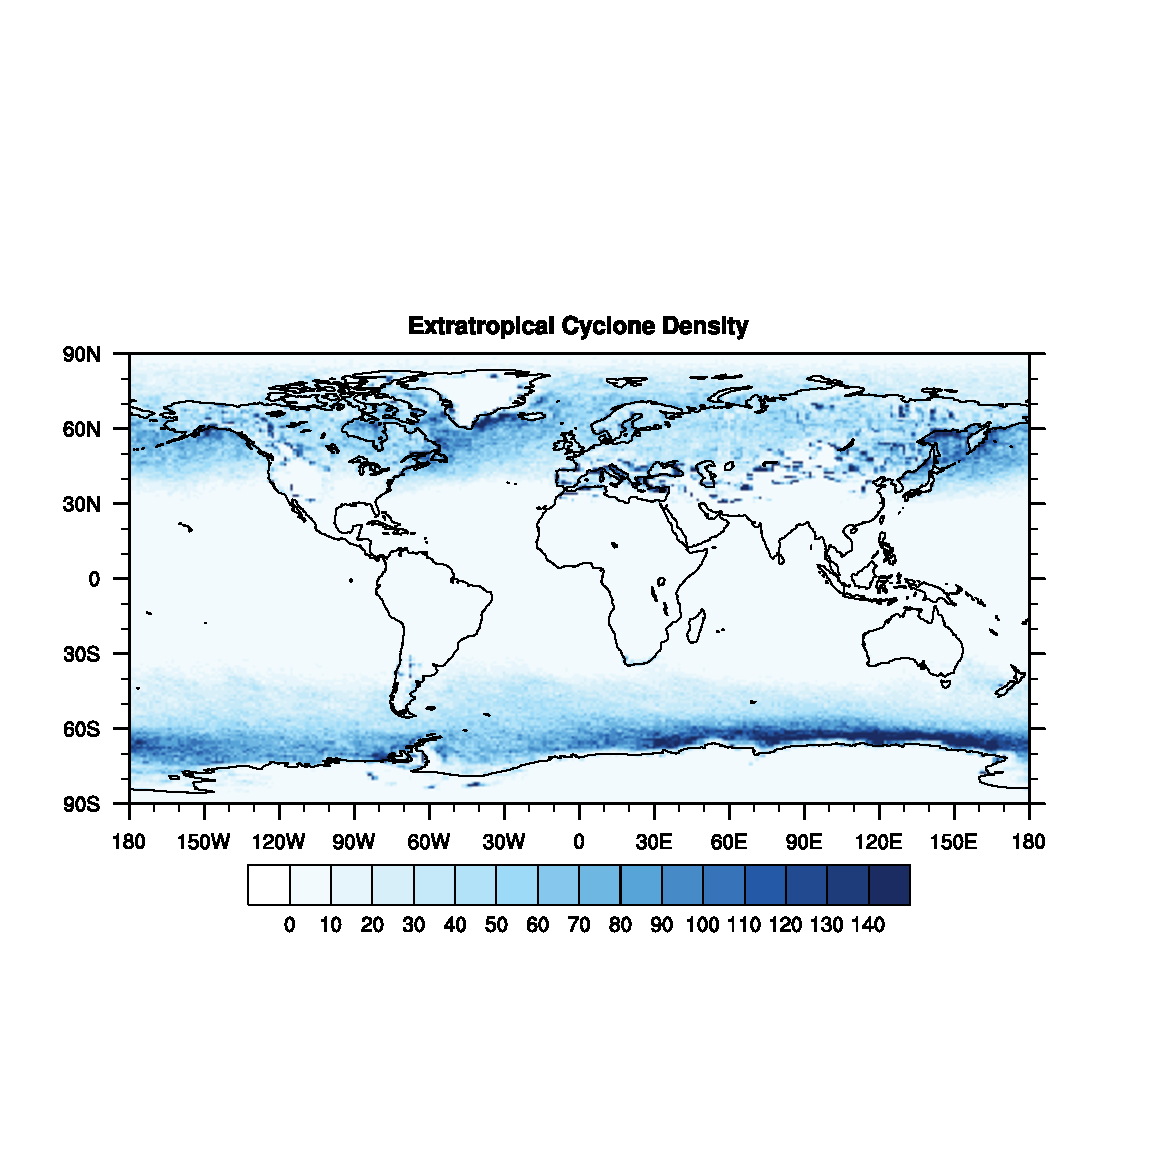
\includegraphics[trim=0.5cm 3.5cm 1cm 4.5cm, clip=true, width=5in]{density_plot}
%\hline
%\end{tabular}
\end{center}
\caption{Extratropical cyclone counts from a 20-year CLIVAR climatological simulation, as obtained by selecting only pressure minima that (a) do not have an upper level warm core, (b) are within 4 degrees of a vorticity maximum, (c) are present over topography of maximum elevation 1500\ m, (d) are persistent for at least 2 days, (e) increase in pressure by  at least 0.1\ hPa over a distance of 1 degree in all directions, and (f) are in the latitude interval [90S, 20S] or [20N, 90N].} \label{fig:DensityPlot}
\end{figure}

\begin{figure}[p]
\begin{center}
%\begin{tabular}{|p{4in}|}
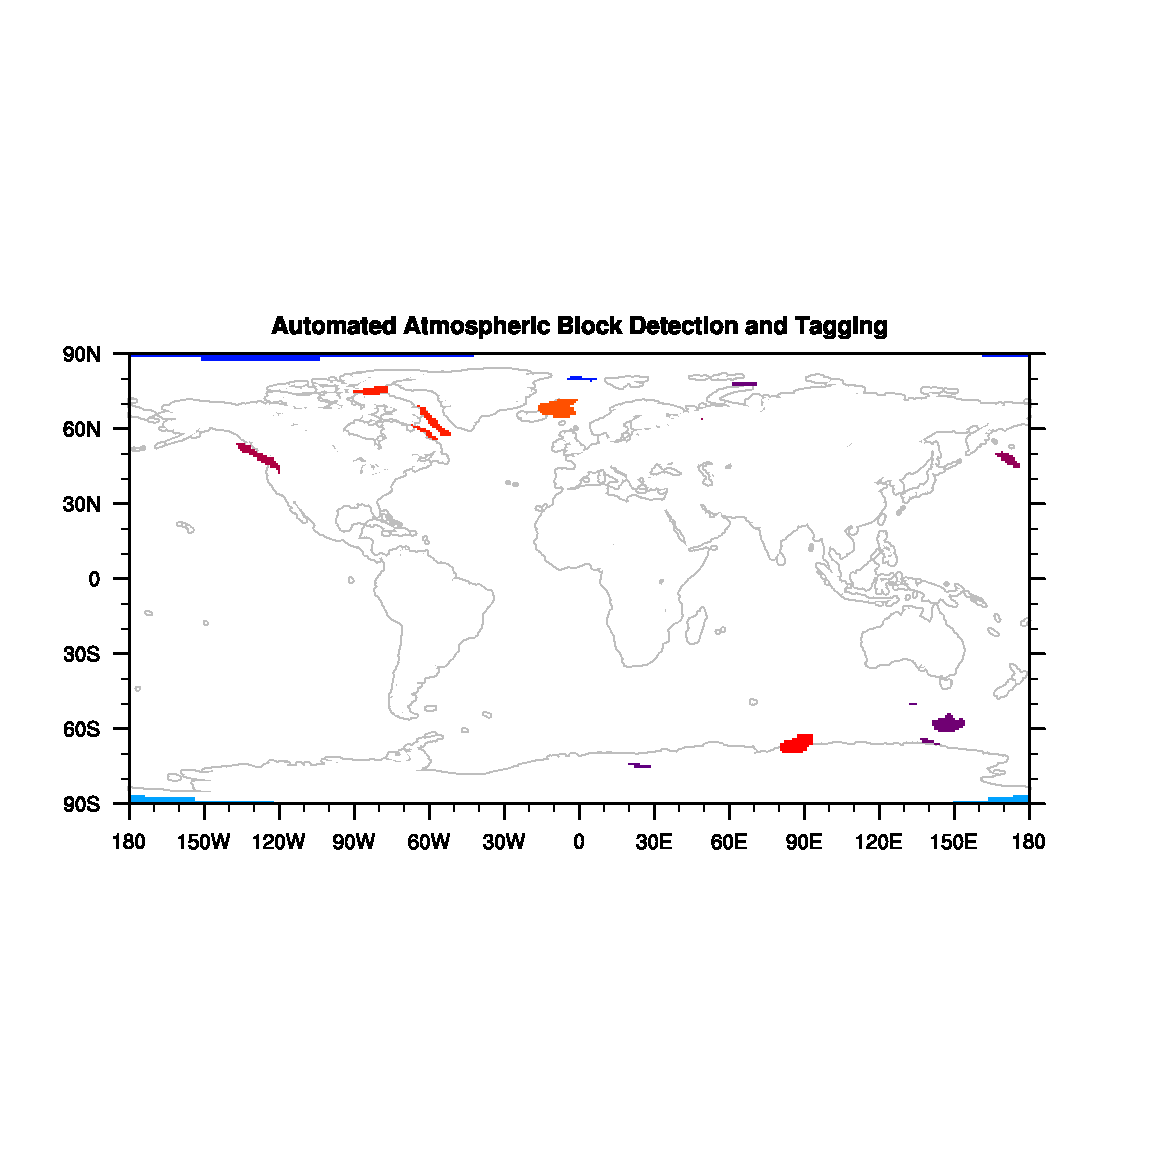
\includegraphics[trim=0.5cm 4.5cm 1cm 4.5cm, clip=true, width=5in]{blob_plot}
%\hline
%\end{tabular}
\end{center}
\caption{Anti-cyclonic column-integrated potential vorticity (PV) anomalies (against a 15 year monthly averaged background state taken from 1979 to 1993), identifying regions where the column integrated PV is less than $-1.3$ PVU (northern hemisphere) and greater than $+1.3$ PVU (southern hemisphere).  This criteria for blocking event detection is described by \cite{scherrer2006two}, as applied to the ERA-Interim reanalysis data for 11 June 2005.  Discrete blocking events are tagged with a unique identifier based on spatial and temporal connectivity.} \label{fig:BlockingDetection}
\end{figure}

\subsubsection{Atmospheric blocks}

Various algorithms have been developed in the literature for the identification of blocking events in atmospheric model data \citep{tibaldi1990operational, wiedenmann2002climatology, pelly2003new, schwierz2004perspicacious, scherrer2006two, tyrlis2008aspects, barriopedro2010application, barnes2012methodology}, and most of these approaches use either geopotential height, 500mb velocity or potential vorticity as indicators (with a variety of thresholds).  However, robust algorithmic detection of atmospheric blocking events has been particularly difficult due to the fact that atmospheric blocking manifests in many different forms \citep{haby2008blocking}, such as Rex Blocks, Omega Blocks, etc.  Notably, the focus of the majority of past studies has also been on Euro-Atlantic blocking, with only a few studies assessing atmospheric blocking over North America.  Assessing blocking indices over North America will be a major focus of this proposal.

%{\color{red}[What about the blocking indicator papers?]}
No prior analysis has examined trends in atmospheric blocking based on tracking and characterizing discrete blocking episodes, and existing work that uses diagnosed dynamical quantities are largely limited to a single dataset of characterization.  In \cite{croci2007multifaceted}, ERA-40 reanalysis was used to document an observed decrease in blocking over Greenland and the North Pacific.  Others have claimed that the duration of blocking events and associated heat waves may increase under global warming \citep{lupo1997climatological, beniston20042003}.  However, recent work by \cite{barnes2012methodology} observed that, using 500mb wind speed as an indicator and data from the CMIP5 dataset, duration of blocks remained roughly constant whereas frequency decreased.  \cite{dandrea1998northern} compared atmospheric blocking events from 15 atmospheric general circulation models and found that models at the time tended to underestimate both blocking frequency and the average duration of blocks.

%Consequently, it is anticipated that global detection of blocking events will require a multi-pronged approach.  In order to manage all sets of input data, a combination of processing methods using Python scripts and C++ will be used for handling of reanalysis data and CESM output.  Idealized tests to verify correct behavior of this algorithm will use the idealized baroclinic instability test with potential vorticity tracer proposed by \cite{JPWCJJKRBR2013QJRMS}.  Each detection algorithm will be applied to the reanalysis datasets to determine which formulation provides the most robust approach for detection of both northern hemisphere and southern hemisphere blocking events.  Preliminary results showing regions of anti-cyclonic column-integrated potential vorticity (PV) anomalies using a detection approach analogous to \cite{scherrer2006two} are shown in Figure \ref{fig:BlockingDetection}.

\subsubsection{Atmospheric rivers}

Algorithms for detection of ARs generally use their basic properties \citep{ralph2011storms}, including (a) an integrated column water vapor of 2 cm, (b) wind speeds greater than 12.5 m/s in the lowest 2 km and (c) a long, narrow shape of length at least 2000 km and width less than 1000 km.  This definition is typically augmented algorithmically via image processing techniques such as edge detection, for identifying the structure of the event \citep{wick2013description}.  Other algorithms include \cite{zhu1998proposed, bao2006interpretation, dirmeyer2007characterization, gimeno2010origin, lavers2012detection}.   Notably, detection algorithms have had some difficulty assessing point of landfall, possibly attributed to insufficient model resolution \citep{wick2014implementation}.

\subsubsection{Temperature extremes}

{\color{red}[More here]}

This task seeks to implement and analyze several algorithmic approaches for the detection and characterization of heat waves and cold spells.  Part of the goal of this work will be to determine if detection indicators of heat waves are correlated with typical indicators for blocking events in the reanalysis datasets.  An analogous study was performed \cite{della2007summer}, which examined summer heat waves over western Europe over the 20th century and showed that many European heat waves are correlated with anomalous high pressure systems over Scandinavia characteristic of an atmospheric blocking event.  This proposal aims to expand this study to the global scale using the previously developed framework of multiple reanalysis datasets and detection algorithms.

{\color{red}[Use apparent temperature?]}

\subsubsection{Precipitation extremes}

{\color{red}[More here]}

This task seeks to implement and analyze several algorithmic approaches for the detection and characterization of precipitation extremes, with a focus on precipitation extremes.

\subsubsection{Visualization}

This proposal aims to produce maps of changing extreme weather density over North America, along with informational labels identifying changes in characteristics that will affect key regions and sectors.  {\color{red}[More]}  Box plots showing changes in characteristics when breaking the sample period into two.

\subsection{Research Tasks}

%\subsubsection{Climate Indicators}

%This project will provide an assessment of changes in many of the characteristics of extreme weather events.  Under this umbrella we include an assessment from key NASA datasets, plus two projects ``assessing human-induced climate change'' and ``projecting future change.''

%To support future assessment capabilities, this project further seeks to integrate the TempestExtremes package in the NASA Earth Exchange (NEX) to allow for high-throughput analysis of submitted datasets from other NEX users.

\subsubsection{(T1) Implementation of new detection and characterization algorithms} \label{sec:T1}

This research task will focus on the implementation and testing of several new detection and characterization algorithms in the TempestExtremes framework, augmenting the existing set of  algorithms.

\paragraph{ETCs and TCs:}  A flexible algorithmic framework has already been developed for ETCs and TCs, as described in section \ref{sec:Methods}.  No additional modifications are planned as part of this proposal.

\paragraph{Atmospheric Blocks:}  Two methods for blocking detection have already been implemented in TempestExtremes:  specifically, \cite{schwierz2004perspicacious}, using column integrated potential vorticity, and \cite{pelly2003new}, using a blocking indicator based on Rossby wave overturning.  We will augment these algorithms with methods based on \cite{tibaldi1990operational} that uses the gradient of geopotential height to detect flow reversal.

\paragraph{Atmospheric Rivers:}  This proposal aims to implement the method of \cite{jiang2014intermediate}, which is based off of the definition of \cite{ralph2004satellite} and incorporates a number of modern features of AR detection algorithms.  AR structures will be agglomerated in space using a graph traversal algorithm, and then connected in time by determining overlaps in detections at adjacent time points.

\paragraph{Heat Extremes:}  {\color{red} [More needed]}

\paragraph{Precipitation Extremes:}  {\color{red} [More needed]}

\subsubsection{(T2) Assessment of lagging indicators} \label{sec:T2}

The climate indicator focus of this proposal will assess past trends in the characteristics of extreme weather events that have been enumerated in section \ref{sec:ExtremeWeather}.  This will be the first comprehensive study of discrete extreme weather events in reanalysis data, and will lead to a catalogue of events and associated characteristics.  Reanalysis products, as described in section \ref{sec:Datasets} will be key to assess past changes, including the Modern Era Retrospective-analysis for Research and Applications (MERRA), CFSR, ERA-Interim and North American Regional Reanalysis (NARR) (for all extreme events), Daymet (for temperature and precipitation extremes) and PRISM precipitation data (for precipitation extremes).  CMIP5 hindcast simulations will be used to determine if observed trends in the characteristics of extremes also appear in standalone climate model simulations with prescribed SSTs.  This project will also require the development of a pre-processing codebase that is capable of transforming input climate data into a single standard compatible with TempestExtremes.  In addition, the following special topics will be tackled by this work:

\paragraph{Tropical Cyclones:}  Atmospheric reanalysis data (MERRA and CFSR) will be used in conjunction with the International Best Track Archive for Climate Stewardship (IBTrACS) tropical cyclone best track database \citep{Knapp2010} to assess the performance of commonly-used tracking parameter combinations. Sensitivity tests which perturb the thresholds used to define tropical cyclones in climate data will be completed to assess whether or not the storm detection process is highly sensitive to the choice of specific criteria.

\paragraph{Extratropical Cyclones:}  Accurate detection of ETCs over high topography, such as the Rocky Mountains, remains an outstanding question that will be studied with this work.  This issue has been an obvious hurdle in the ETC community \cite{neu2013imilast}, but the impacts of winter storm systems on communities throughout North America require accurate knowledge of possible trends in storm tracks.

%(ETC2) The extratropical transition for TCs \cite{hart2001climatology} will be studied in the context of TC detection -- in particular, we are interested in determining if there has been any shift in the mean location of the extratropical transition, as a TC transitions from a warm-core storm to a cold-core ETC.  (ETC3) Recent work by {\color{red}Wehner et al.} has 

%Again a number of approaches will be studied and tuned using a suite of reanalysis data, and verified using multiple datasets and a visual intercomparison.  In particular, we will verify that historically relevant extratropical storms are correctly detected and characterized by the algorithm.


%Studies of extratropical cyclones under future climate scenarios suggest that the expansion of the Hadley circulation will drive extratropical cyclones poleward \citep{bengtsson2006storm} and the warmer climate will lead to an intensification of precipitation of these storms \citep{bengtsson2009will, zappa2013multi}.

%This proposal will address the issue of whether observed intensification over the southern hemisphere in reanalysis data is corroborated with model results, or is likely associated with an increase in the number of observing stations \citep{simmonds2000variability}.  This work will also address the question of attribution of changes in ETCs to anthropogenic forcing, a question which has not yet been tackled in the literature.

\paragraph{Atmospheric Blocks / Heat Waves:}  This proposal aims to determine if detection indicators of heat waves are correlated with typical indicators for blocking events in reanalysis.  It has been shown that summer heat waves over western Europe over the 20th century are correlated with anomalous high pressure systems over Scandinavia characteristic of an atmospheric blocking event \cite{della2007summer}.  This proposal aims to expand this study to the North America using the previously developed framework of multiple reanalysis datasets and detection algorithms.

%This proposal aims to compare the three algorithmic approaches for identifying and characterizing atmospheric blocking events and determine any trends associated with block intensity (for instance, measured in terms of potential vorticity anomaly if using the indicator of \cite{schwierz2004perspicacious}), lifetime, genesis location and track.  Particular emphasis will be paid to detection algorithms that are capable of detecting blocking over North America.

%\paragraph{Atmospheric Rivers:}  Discrete AR events will be characterized in terms of point of landfall and total associated precipitation (rainfall and snowfall), analogous to characterizations of \cite{neiman2008meteorological} and \cite{guan2010extreme}.  Statistics will then be computed on these quantities including proportion of precipitation associated with AR events, frequency of AR events and mean spatial point of landfall.  MERRA and CFSR data will be used for this assessment.

%{\color{red}Correlations between extremes?}

%{\color{red}[More work needed here]} This task aims to perform the first comprehensive study of blocking events and ETCs in historical reanalyses data, including the NCEP, ERA-40, MERRA and C20C datasets.  Using the detection algorithms developed in Task 1, this proposal aims to determine historical counts of blocking events / ETCs and differences between the event characteristics obtained from each reanalysis dataset.  A particular focus in this analysis will be given to extreme value statistics (how does the return time of extreme blocking events vary by region), which are associated with blocking events / ETCs that have the potential for the most socioeconomic damage.  Properties specific to blocking events that will be considered include intensity, duration, classification, return time and associated weather.  Those specific to ETCs include wind intensity (in terms of vorticity, minimum sea-level pressure or gradient of sea-level pressure), radius of maximum winds, intensity of precipitation, latitude of genesis point, latitude of termination and probability of transit beyond a given latitude.  This task will tackle the question of how these characteristics can be filtered from each dataset once a successful detection has been obtained.  To do so, this work will rely on both past surveys of event characteristics \citep{serreze1995climatological}, as well as building an understanding of the general features of ETCs in historical reanalysis data.

\subsubsection{(T3) Assessing Human-Induced Climate Change (Attribution)} \label{sec:T3}

The question of the influence human activity on the frequency and magnitude of extreme weather events of the past decade has remained largely unanswered.  To address this question, this proposal will apply the TempestExtremes suite of detection and characterization algorithms to the ensemble of ``world that was'' and ``world that could have been'' simulations from the C20C (see section \ref{sec:Datasets}).  By contrasting extreme weather events within these two datasets, anthropogenic influences can be separated from natural variability. These ensemble runs enlarge the statistical sample of extreme events, which are inherently rare. These data can be further used to analyze the time series of observation-based historical data and improve estimates of probability / frequency distributions for extreme events with specific characteristics.

%Since this second set of simulations arise from a world without anthropogenic forcing, differences in the statistics of blocking events and ETCs can be effectively attributed to anthropogenic drivers.  Consequently, this study aims to look at how the statistics of blocking events have changed under human influence (such a study is known as detection and attribution).

%As part of the Climate of the 20th Century (C20C) project, 100 climate simulations have been produced covering the period 1959-2011, half representing a climate consistent with known greenhouse gas emissions and sea-surface temperatures, and half representing conditions with anthropogenic forcing removed.  

The results of this task would also provide enlightenment on specific atmospheric events of the past (other such studies include \cite{stott2004human} and \cite{pall2011anthropogenic}).  Namely, it would address questions such as ``what was the probability of the 1993 Storm of the Century in a world with and without anthropogenic forcing?''  Statistically significant differences between the probability in the forced and unforced simulations in 1993 would lead to conclusions on the influence of human activity on the likelihood of these events.  The large ensemble (50 members) that will be leveraged as part of this project is necessary in order to provide accurate statistics on relatively infrequent events such as these, and so this proposal is uniquely positioned to answer these questions.

%Past studies also do not address how the characteristics of general blocking events have been modified (or will be modified) by anthropogenic influences, and cannot provide a statistical assessment of how much the extreme heat wave events of the past decade can be attributed to human-induced changes.  The proposed work will assess trends in blocking from a number of datasets, using multiple dynamical indicators, and will use large-ensemble experiments to attribute changes in blocking to human influences.

%\subsubsection{(T4) Assessment of leading indicators (future change)}

\subsubsection{(T4) Integration of the Extreme Weather Pipeline in NEX} \label{sec:T4}

\begin{figure}
\begin{center}
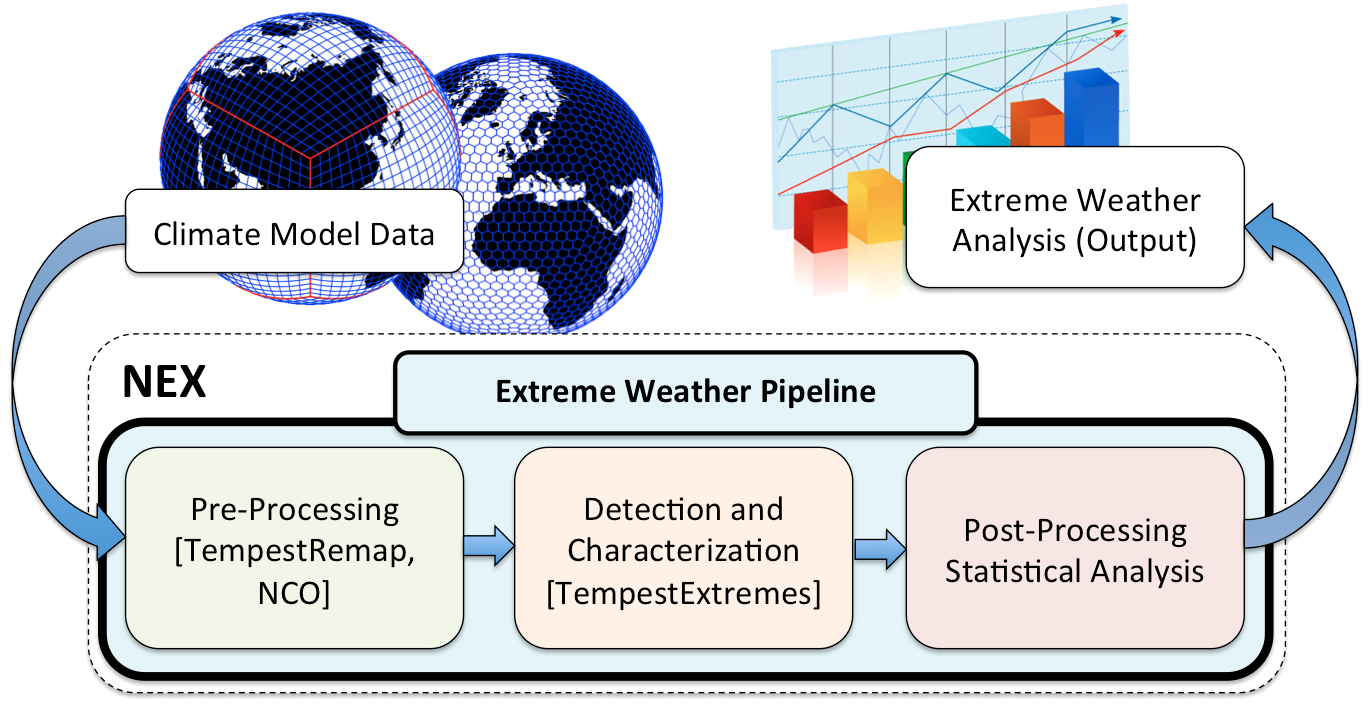
\includegraphics[width=5in]{TempestPipeline.png}
\end{center}
\caption{A depiction of the Extreme Weather Pipeline for supporting analysis of climate data through the NEX system.} \label{fig:TempestPipeline}
\end{figure}

We propose the integration of the TempestExtremes detection and characterization software into the existing NASA Earth Exchange (NEX) infrastructure, to provide a capability for scientists to quickly obtain information and statistics on extreme weather events from their climate datasets.  A depiction of the software pipeline exposed to climate scientists is shown in Figure \ref{fig:TempestPipeline}.  First, gridded climate data and grid metadata are provided to the pre-processor so as to convert the data to a format compatible with the detection and characterization toolset.  This step entails both regridding of the climate data to a latitude-longitude grid and computation of additional diagnostic variables (for instance, computation of vorticity from wind vectors).  The processed input data is then fed into the detection and characterization software (TempestExtremes), where the user has the capability to specify the set of extreme weather events to identify and their characteristics (indicators) of interest.  Multiple detection algorithms (even for the same extreme weather event) or parameter choices can be specified at this stage.  The results of the detection and characterization step is then fed into a statistical post-processor, where the user again has the option of computing statistical quantities of interest.

The software associated with this proposal will be implemented using C++.    Execution of the code will be performed on NASA's computing systems via the NEX interface.  Integration of the software product with NEX will involve direct collaboration with Weile Wang and Ramakrishna Nemani, leads on the NEX project.

%\subsubsection{Visualization}

%\subsubsection{Future Efforts}

%Two options are available for providing projections of future change: static climatologies produced via Climate Variability and Predictability (CLIVAR) experiments under doubled atmospheric CO$_2$ and/or increased sea-surface temperatures, and dynamic climatologies obtained from the CMIP5 multi-model multi-ensemble database.

\subsection{Management Plan and Timetable of Activities} \label{sec:Timeline}

PI Ullrich will provide leadership for this project and coordinate activities for atmospheric blocks and ARs.  Co-PI Grotjahn will coordinate activities for temperature and precipitation extremes and provide advisement on activities for atmospheric blocks.  Co-I Zarzycki will coordinate activities for TCs, and will provide advisement on activities for ETCs.  PI Ullrich will also be in charge of coordinating software development and ensuring that this work meets the necessary software engineering guidelines.  Each of the graduate student researchers involved in this project will work on three of the atmospheric features presented in this proposal, although it is anticipated that there will be substantial collaboration on the technical level.  Communication between partners will be managed via telecon, one annual meeting at UC Davis between all project members, and once annually at the American Geophysical Union Fall Meeting.

The approximate timeline of the research component of this proposal is as follows:  The first year will be dedicated towards the development of new detection and characterization algorithms (section \ref{sec:T1}).  Characterization and assessment of trends in these indicators is the major focus of this project, and will cover a 2.5 year period (section \ref{sec:T2}).  This task involves assessments of reanalysis data, gridded data and CMIP5 hindcast data.  The attribution study (section \ref{sec:T3}) will be carried out beginning in year 2 and will proceed through the beginning of year 3.  Finally, NEX integration (section \ref{sec:T4}) will be carried over the last half of the project as the codebase converges on a specific suite of algorithms.  This timeline is summarized in Table \ref{tab:ExpectedTimeline}.

\begin{table}
\begin{tabular}{l||c|c|c|c||c|c|c|c||c|c|c|c|}
& \multicolumn{4}{c}{Year 1} & \multicolumn{4}{c}{Year 2} & \multicolumn{4}{c}{Year 3}  \\
\hline
         & 1st & 2nd & 3rd & 4th & 1st & 2nd & 3rd & 4th  & 1st & 2nd & 3rd & 4th \\
\hline
\hline
(T1) Detection algor. & \cellcolor{red!35} & \cellcolor{red!35} & \cellcolor{red!35} & \cellcolor{red!35} & & & & & & & &  \\
\hline
(T2) Indicators  & \cellcolor{green!35} & \cellcolor{green!35} & \cellcolor{green!35} &  \cellcolor{green!35}  & \cellcolor{green!35} & \cellcolor{green!35} & \cellcolor{green!35} & \cellcolor{green!35} & \cellcolor{green!35} & \cellcolor{green!35} & & \\
\hline
(T3) Attribution study & & & & & \cellcolor{blue!35} & \cellcolor{blue!35} & \cellcolor{blue!35} &  \cellcolor{blue!35}  & \cellcolor{blue!35} & \cellcolor{blue!35} & & \\
\hline
(T4) NEX Integration  & & & & & & & \cellcolor{cyan!35} &  \cellcolor{cyan!35}  & \cellcolor{cyan!35} & \cellcolor{cyan!35} & \cellcolor{cyan!35} &  \cellcolor{cyan!35} \\
\hline
\end{tabular}
\caption{Expected timeline of (split in quarters for each year) for all major activities.} \label{tab:ExpectedTimeline}
\end{table}

We anticipate that multiple major peer-reviewed publications will arise from this work, addressing the studies of detection, attribution and prediction. Further, this work will be presented at major scientific meetings, including the annual meetings for the American Meteorological Society, the Americal Geophysical Union, and the International Association of Meteorology and Atmospheric Sciences.  A final report will be developed as part of this proposal summarizing the conclusions drawn from this work along with advice for future research directions.

\clearpage

\section{References and Citations}

\vspace{-1cm}
\bibliography{Ullrich-NASAIndicators-Bibliography}
\bibliographystyle{plain}

\clearpage

\includepdf{Ullrich-Biographical.pdf}
\includepdf{Zarzycki-Biographical.pdf}

\clearpage

\section{Current and Pending Support}

\subsection{PI Ullrich}

\subsubsection{Current}

\begin{tabular*}{\textwidth}{@{\extracolsep{\fill}}lp{5.5in}}
Title: & Identifying the Influence of Anthropogenic Forcing on Extreme Weather Events \\
PI: & P. Ullrich \\
Agency: & Hellman Foundation \\
PI months/year: & 1.0 \\
Dollar value: & \$30,000 \\
Period: & 1 August 2014 -- 31 July 2015
\end{tabular*}

\begin{tabular*}{\textwidth}{@{\extracolsep{\fill}}lp{5.5in}}
Title: & Multiscale Methods for Accurate, Efficient, and Scale-Aware Models of the Earth System (Supplement) \\
PI: & W. Collins \\
Agency: & Department of Energy \\
PI months/year: & 1.0 \\
Dollar value: & \$80,000 \\
Period: & 1 August 2014 -- 31 July 2015
\end{tabular*}

\subsubsection{Pending}

\begin{tabular*}{\textwidth}{@{\extracolsep{\fill}}lp{5.5in}}
Title: & Application sector-based climate indicators, from the past into the future \\
PI: & R. Grotjahn \\
Agency: & NASA \\
PI months/year: & 1.0 \\
Dollar value: & \$575,022 \\
Period: & 1 September 2015 -- 31 August 2018
\end{tabular*}

\begin{tabular*}{\textwidth}{@{\extracolsep{\fill}}lp{5.5in}}
Title: & A New Approach for the Computational Needs of Next-Generation High-Resolution Climate Simulations  \\
PI: & P. Ullrich \\
Agency: & National Science Foundation \\
PI months/year: & 1.0 \\
Dollar value: & \$481,735 \\
Period: & 1 July 2015 -- 30 June 2018
\end{tabular*}

\begin{tabular*}{\textwidth}{@{\extracolsep{\fill}}lp{5.5in}}
Title: & Diagnosing and Advancing Scale-Aware Convection Parameterizations for Unified Multi- Scale GCMs  \\
PI: & C. Jablonowski \\
Agency: & Department of Energy Office of Science \\
PI months/year: & 1.0 \\
Dollar value: & \$343,476 \\
Period: & 1 March 2015 -- 29 February 2018
\end{tabular*}

\begin{tabular*}{\textwidth}{@{\extracolsep{\fill}}lp{5.5in}}
Title: & Advancing the Frontiers of Variable and High-Resolution GCMs for Regional Climate Assessments and Extreme Events  \\
PI: & C. Jablonowski \\
Agency: & Department of Energy Office of Science \\
PI months/year: & 1.0 \\
Dollar value: & \$366,738 \\
Period: & 1 September 2014 -- 31 August 2017
\end{tabular*}

\begin{tabular*}{\textwidth}{@{\extracolsep{\fill}}lp{5.5in}}
Title: & Understanding Human Influence on Atmospheric Blocking and Extratropical Cyclones  \\
PI: & P. Ullrich \\
Agency: & Department of Energy Office of Science \\
PI months/year: & 1.0 \\
Dollar value: & \$457,950 \\
Period: & 1 October 2014 -- 30 September 2017
\end{tabular*}

\subsection{Co-PI Grotjahn}

\subsubsection{Current}

\begin{tabular*}{\textwidth}{@{\extracolsep{\fill}}lp{5.5in}}
Title: & Large scale dynamics and statistics of California extreme weather in the atmosphere and in global models  \\
PI: & R. Grotjahn \\
Agency: & National Science Foundation \\
Grant number: & 1236681 \\
PI months/year: & 1.5 (0.5 to be paid) \\
Dollar value: & \$603,843 \\
Period: & 1 October 2012 � 30 September 2015
\end{tabular*}

\subsubsection{Pending}

\begin{tabular*}{\textwidth}{@{\extracolsep{\fill}}lp{5.5in}}
Title: & Synoptic-Dynamics Processes-based Metrics for Hot and Cold Spells Simulations in Climate Models   \\
PI: & R. Grotjahn \\
Agency: & NOAA \\
PI months/year: & 1.5 (0.5/year on average to be paid) \\
Dollar value: & \$442,553 \\
Period: & 1 May 2015 � 30 April 2018
\end{tabular*}

\begin{tabular*}{\textwidth}{@{\extracolsep{\fill}}lp{5.5in}}
Title: & Application sector-based climate indicators, from the past into the future \\
PI: & R. Grotjahn \\
Agency: & NASA \\
PI months/year: & 1.5 (0.5 in years 1 and 3, 1.5 in year 2) \\
Dollar value: & \$575,022 \\
Period: & 1 September 2015 � 31 August 2018
\end{tabular*}

\clearpage

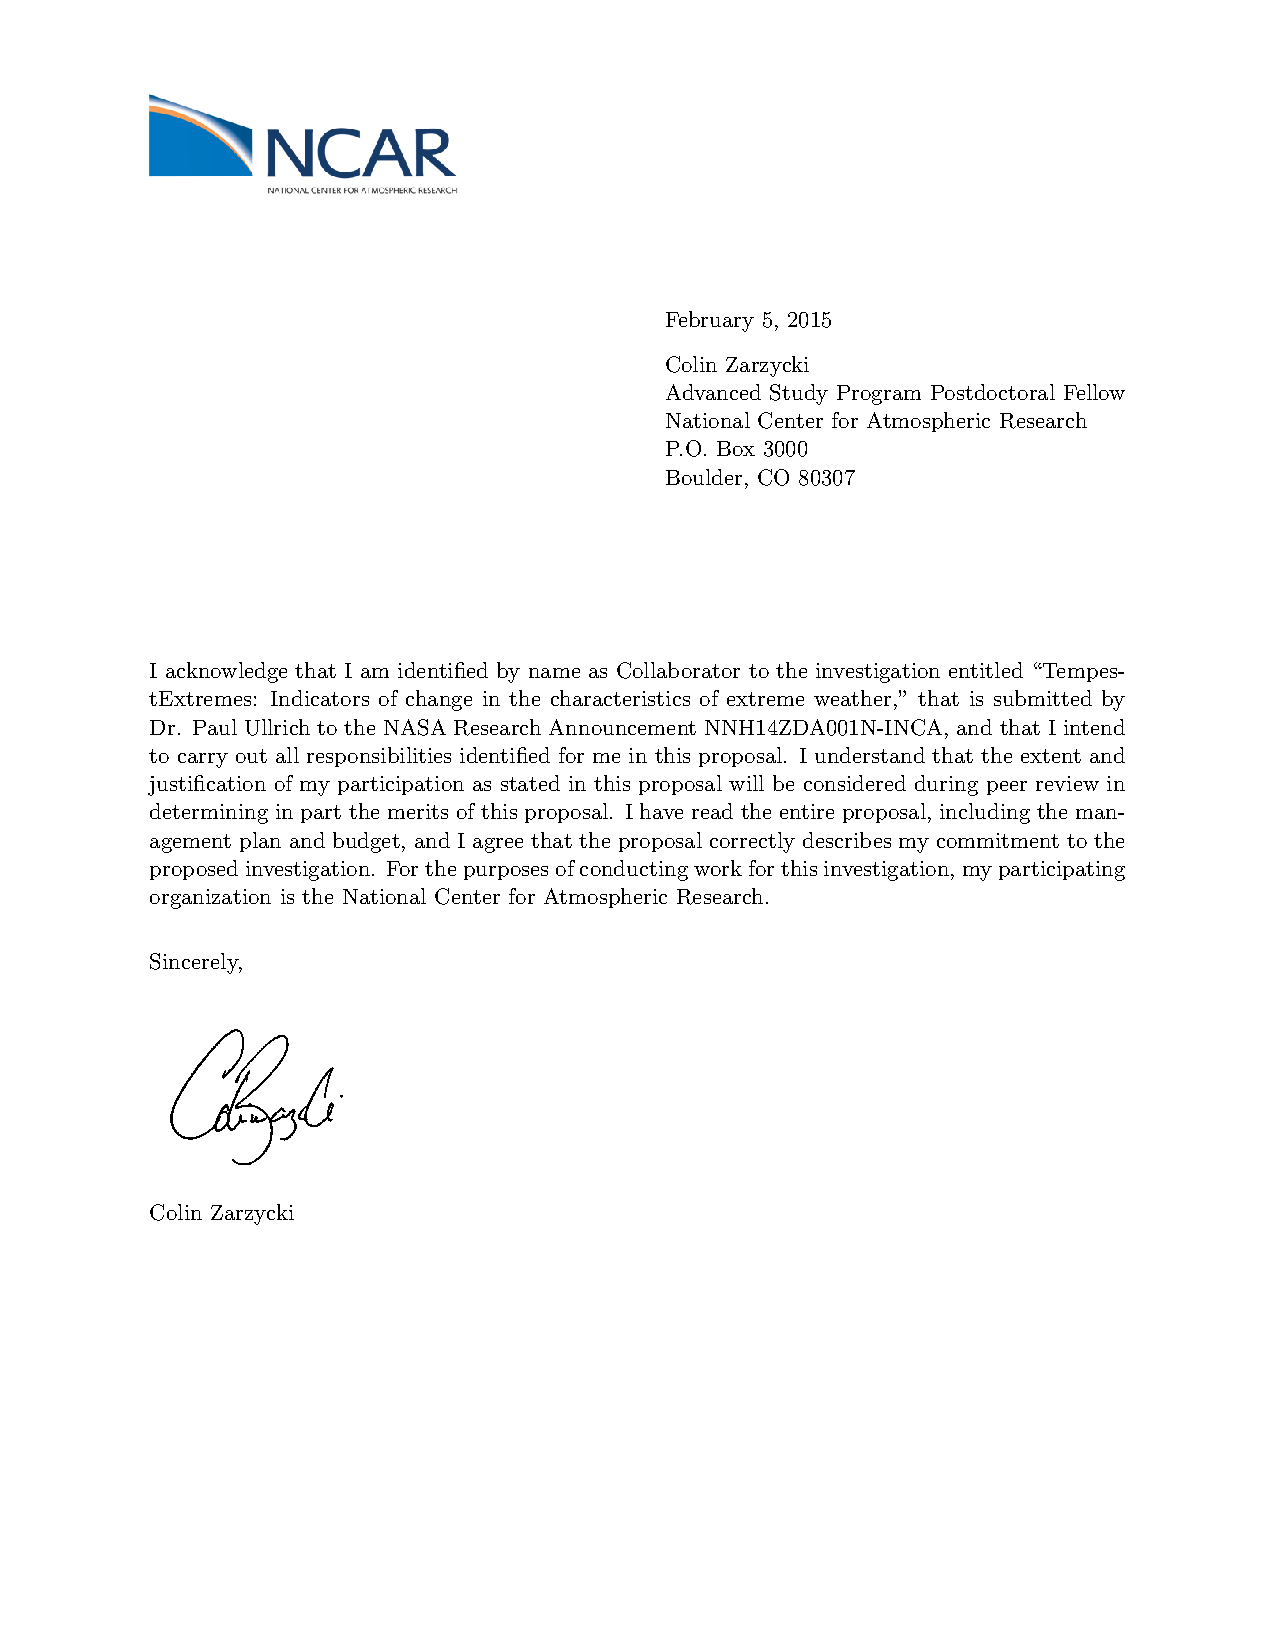
\includepdf{Zarzycki-Letter}
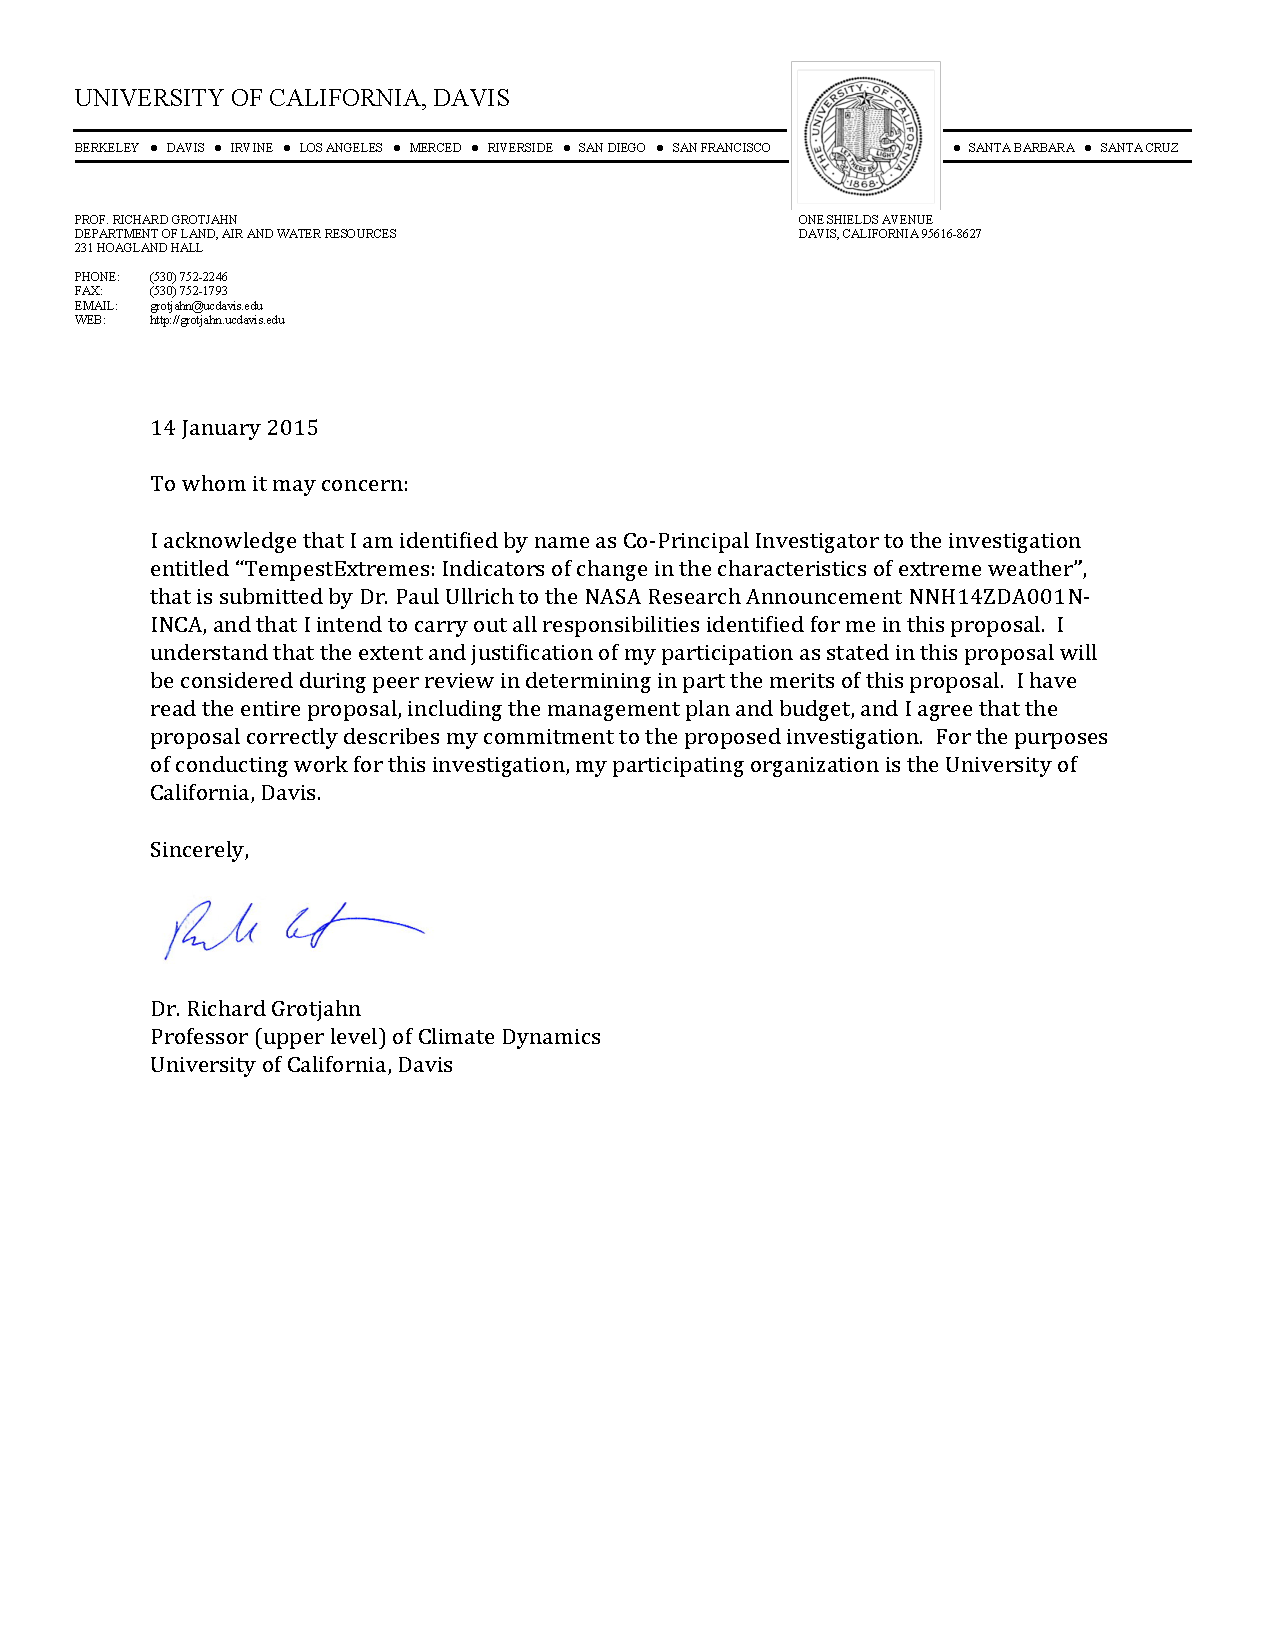
\includepdf{Grotjahn-Letter}

\clearpage

\section{Budget Justification}

\subsection{Personnel (\$235,583)}
Salaries are based on Fiscal Year 2014/2015 levels and assume a 3\% increase in each subsequent fiscal year.

\subsection{Salaries (\$224,812)}

\subsubsection{Principal Investigator (Dr. Paul Ullrich) \$25,333}

PI Dr. Paul Ullrich will be direct charging the project 1 month (8.33\% of his annual effort) of salary in project years 1, 2 and 3. Anticipating a forthcoming merit increase, this amounts to salary costs of \$8,196 in year 1, \$8,442 in year 2 and \$8,695 in year 3. 

\subsubsection{Co-Principal Investigator (Dr. Richard Grotjahn) \$22,093}

co-PI Dr. Richard Grotjahn will be direct charging the project a ? month of salary (4.17\% of his annual effort) in project years 1, 2 and 3. This amounts to salary costs of \$7,148 in year 1, \$7,362 in year 2 and \$7,583 in year 3. 

\subsubsection{Graduate Student Researcher IV (TBN x2) \$177,386; \$88,693 each}

Two graduate student researchers (GSR IVs; 9 months at 48\%, 3 summer months at 100\%) will be funded for the duration of this project, conducted as part of their degree with a thesis option. The current annual salary rate for a GSR IV is \$45,300.  Based on 9 months at 48\% and 3 months at 100\% this amounts to a total of \$57,390 (\$28,695 each) in project year 1, \$59,112 (\$29,556 each) in year 2 and \$60,884 (\$30,442 each) in year 3.

\subsection{Benefits  (\$10,771)}
 
Employee Benefits are based on Federally Approved Composite Benefit Rates. The University of California�s current Composite Benefit Rates have been federally reviewed and approved through June 30, 2015.  Rates for Fiscal Years 2015/2016 and 2016/2017 are projected while the rates for Fiscal Year 2017/2018 and beyond are estimates using a 3\% increase over the preceding year�s rates as the basis of the estimate. 

\subsubsection{Principal Investigator (Dr. Ullrich): \$4,522}
 
As the direct charging of salary for Dr. Ullrich is during the summer of each project year, the projected composite benefit rates are 17\% and 18\% for project years 1 and 2 respectively and an estimated rate of 18.5\% in year 3.
 
 \subsubsection{Co-Principal Investigator (Dr. Richard Grotjahn): \$3,943}
 
As the direct charging of salary for Dr. Grotjahn is during the summer of each project year, the projected composite benefit rates are 17\% and 18\% for project years 1 and 2 respectively and an estimated rate of 18.5\% in year 3.
 
\subsubsection{Graduate Student Researcher IV (TBN x2): \$2,306 (\$1,153 each)}
The composite benefit rate for the GSR is expected to remain at 1.3\% for the duration of the project.

\subsection{Travel}
The budget includes domestic travel costs associated with three annual trips to the American Geophysical Union (AGU) Fall Meeting in San Francisco, CA for the PI and two graduate students. Including registration fees, travel expenses and meal and incidental expenses, the total cost is estimated at \$1,400 per traveler per year. Domestic travel expenses are also included for the PI to present at the American Meteorological Society (AMS) 30th annual Climate Variability and Change conference, to be held in January 2018, estimated at \$2,300 in year 3. International travel expenses are included to the International Association of Meteorology and Atmospheric Sciences (IAMAS) conference in Cape Town, South Africa, to be held in 2017, estimated at \$4,400 for one participant.

\subsection{Supplies: \$6,277}
A one-time expense of \$3,550 will cover the cost of 50 TB in external hard drives to store reanalysis and model data that is generated or utilized by this project.  Additionally the project requires the purchase of software licenses totaling \$2,727.  The software license charges are \$138 / year / license for the mathematics software package Maple and \$165 / year / license for the software package Matlab, for a total of \$303 / year / license. Software will be provided to the GSRs (2 licenses) and PI (1 license) over the duration of the project. This amounts to \$909 / year for all licenses. These software packages will be used by the students and PI for data processing, analysis and modeling.

\subsubsection{Consultant}
Colin Zarzycki of the National Center for Atmospheric research will be brought onto the project in a consultant capacity.  In conjunction with his participation \$2,650 per year covering his annual travel expenses to the American Geophysical Union (AGU) Fall Meeting (\$1,400 per year) and one trip to UC Davis for consultation / in-person meetings (\$1,250 per year) is included. 

\subsection{Other Expenses: \$96,337}

\subsubsection{Publication Charges: \$6,000}

Publication costs are incurred from publication of work produced by this project and the associated annual cost is expected to be \$2,000 per year (16 pages at \$125 per page).

\subsubsection{Tuition and Fee Costs: \$90,337}

The GSR IV is expected to have residency status which amounts to \$27, 292 (\$13,646 per GSR) in year 1, \$30,021 (\$15,010.50 per GSR) in year 2 and \$33,023 (\$16,511.50 per GSR) in year 3.  These totals factor in a 25\% rebate from the Provost and an estimated 10\% increase per academic year.

\subsection{Indirect Cost: \$156,440}

Per the University of California, Davis� Federally approved Indirect Cost Rate for on-campus research, an initial rate of 56.5\% Modified Total Direct Cost will be applied to the project during the period through June 30, 2016 and 57\% for the period of July 1, 2016 through June 30, 2017.  As overhead rates have not been established beyond Fiscal Year 2016/2017 the last approved rate of 57\% is used for the remainder of the project for budgeting purposes.

\end{document}
